\chapter{Propostion: leveraging ROME to replace the relational backend}
\label{sec:leveraging-rome}

The current implementation of Nova is based on a relational database. To enable
Nova to work with several controllers, this database is replicated on each
server hosting a Nova controller, thanks to the Galera project
\footnote{http://galeracluster.com/} The architecture used for the Nova service
has been organised in a way which ensures that each of its sub-services does not
directly manipulate the database: they have an indirect access through a service
called ``nova-conductor" which in turn works with an implementation of the
\textbf{"nova.db.api"} programming interface. Developers of Nova provide an
implementation of this interface that is using \textit{SQLAlchemy} to manipulate
a relational database.

Leveraging the software interfaces provided by \textit{SQLAlchemy}, we developed
the ROME project: it target at delivering a small driver for key/value stores.
We aim at integrating OpenStack Nova with NoSQL backend without modifying
OpenStack's core code. We build a prototype of this driver and made Nova use it
during validations on the Grid'5000 testbed: to develop this prototype we
changed code only in the \textbf{"nova.db.api"} class, to add call to the ROME
driver.

\begin{figure}[h!]
        \centering
        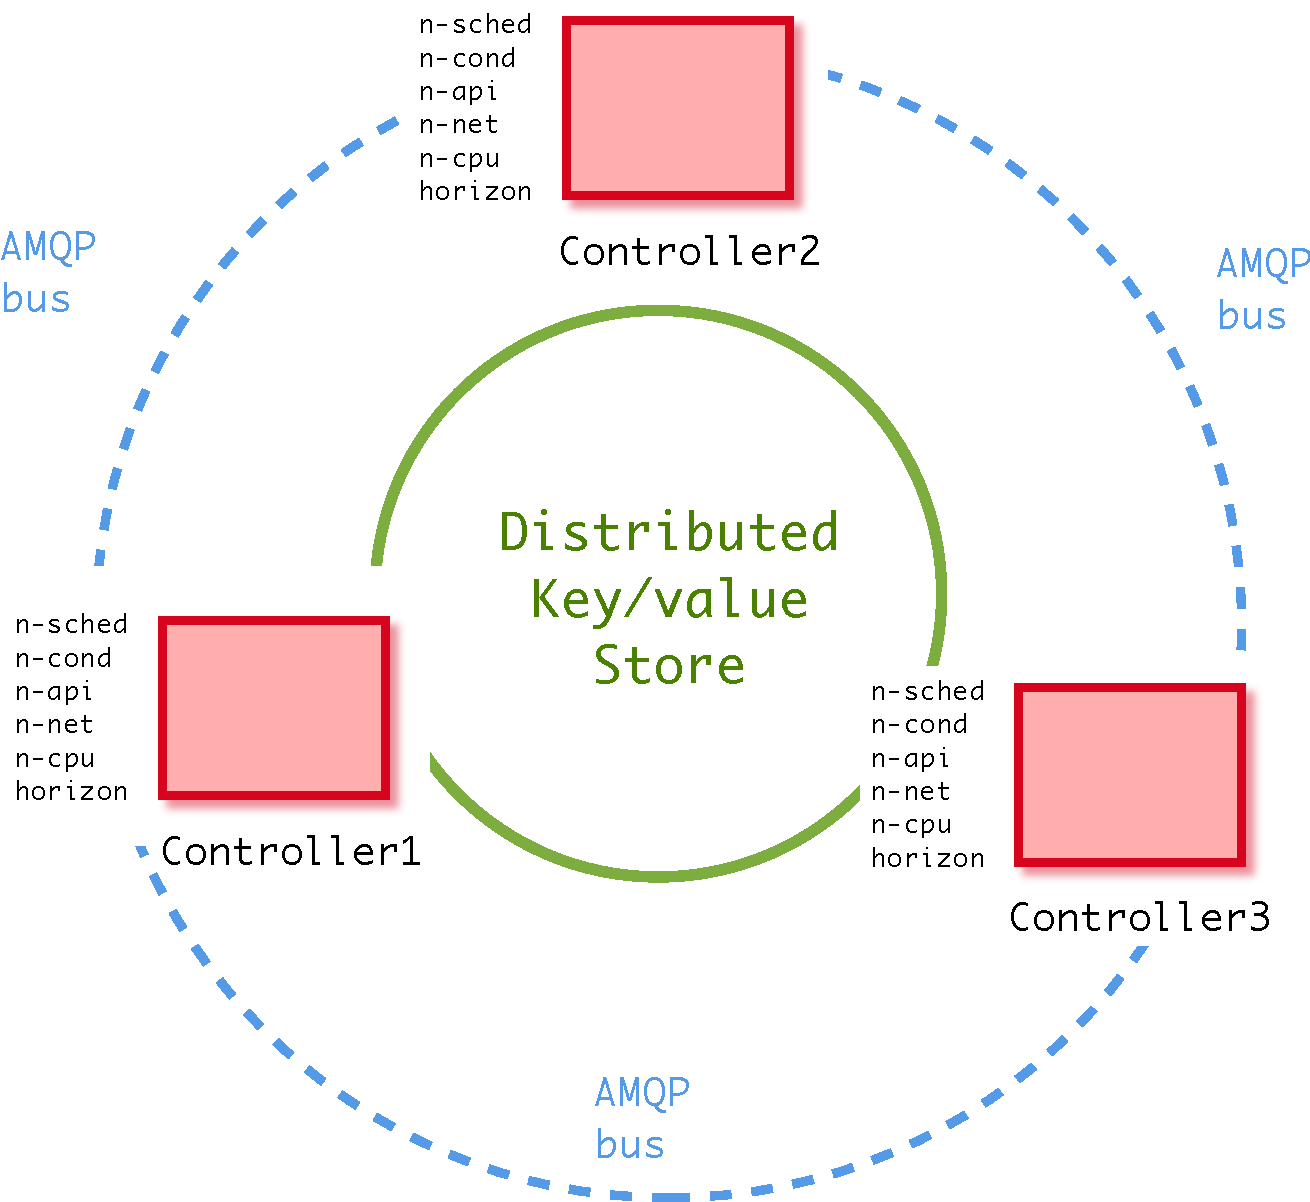
\includegraphics[width=10cm]{figures/OpenStack_distributed.pdf}
        \caption{Nova controllers are connected through a shared key/value backend
        and the AMQP bus.}
      \label{fig:newnova}
\vspace*{-.3cm}
\end{figure}

\section{Mechanisms behind ROME}

Documentation of how to use ROME can be found at:
\textbf{\emph{https://github.com/badock/rome}}

\subsection{How the storage works?}

In order to ensure a compatibility between objects manipulated by the relational
driver and our driver, models leverage the same base class as in the relational
driver. Thus all objects that are supposed to be stored in a non relational
database must extends the \emph{oslo.db.sqlalchemy.models.ModelBase} class which
provides:

\begin{itemize}
\item save function.
\item update function.
\item \emph{"dictionnary like"} behaviour.
\end{itemize}

When an entity object is saved, the ROME driver will marshall it in JSON format:
each of its fields will be translated in JSON value. This transformation is
trivial with integer, string, boolean and lists, but become more complex with
relationships. When the rome driver encounter an object A linked with a remote
object B via a relationship, it will transform the relationship to B with a
\emph{link} object that contains enough information to retrieve the remote
object and then check if b has been modified in order to save its changes. This
mechanisms is illustrated in figure \ref{fig:rome_marshalling}

\begin{figure}[h!]
        \centering
        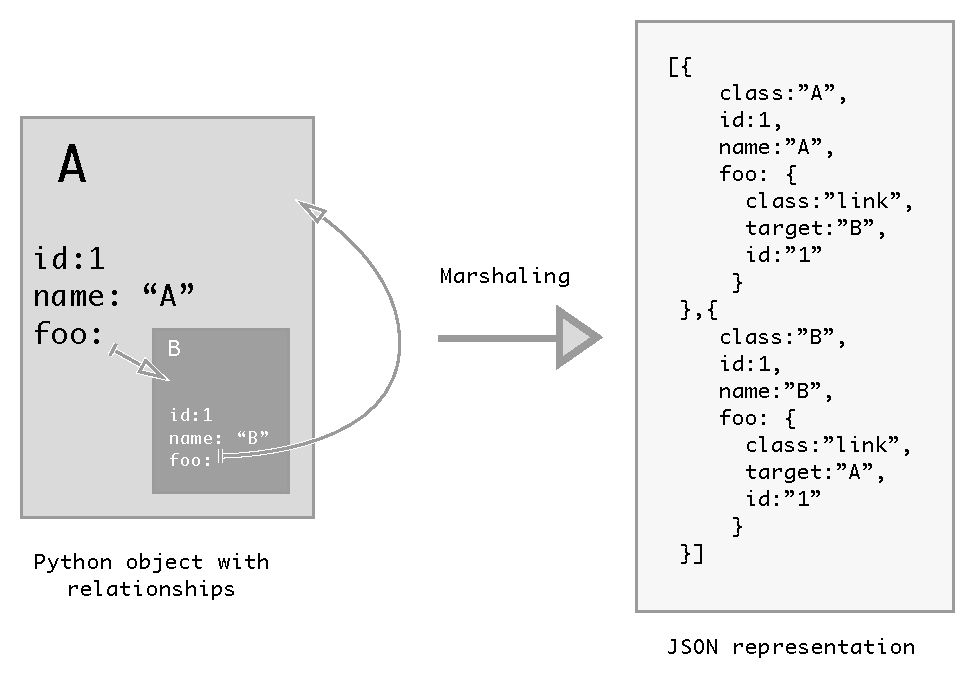
\includegraphics[width=10cm]{figures/rome_marshaling.pdf}
        \caption{An object containing relationships to another object is
        converted to the JSON format and then saved in database.}
      \label{fig:rome_marshalling}
\vspace*{-.3cm}
\end{figure}

Once the object has been marshalled, it can be saved in any KVS \footnote{KVS: Key/value store}: if the KVS support JSON storing, then no transformation is needed,
otherwise it is possible to store the JSON as a string. Keeping a JSON format is
important as it is a widely supported format, which is good for
interoperability.

This JSON data is store in the bucket that corresponds to its original class:
every objects of the same class will be stored in the same bucket.

\subsection{How objects are queried?}

A stored object is associated with a bucket and an id. Thus find an object in
database only consists in identifying its id and its bucket, and then to query
the database for this object.

\begin{figure}[h!]
        \centering
        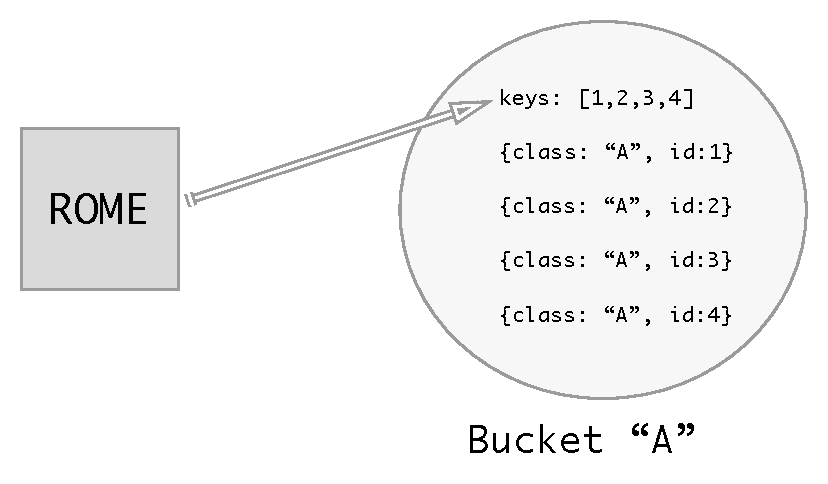
\includegraphics[width=10cm]{figures/rome_query_all.pdf}
        \caption{To query all objects in a bucket, ROME first grab keys of the
        bucket and then query the objects sequentially.}
      \label{fig:rome_marshalling}
\vspace*{-.3cm}
\end{figure}

Querying all objects of a bucket is a bit more complicated: ROME first needs
to get the keys of objects stored in the bucket, and then each object is
sequentially queried. The sequential querying is due to our initial choice for
a KVS backend: RIAK was posing problem when we made parallel access on database
with the python client, thus we decided to tackle this problem later and to
focus on the development of other functions.

